%%%%%%%%%%%%%%%%%%%%%%%%%%%%%%%%%%%%%%%%%%%%%%%
% Template per Elaborato di Laurea
% DISI - Dipartimento di Ingegneria e Scienza dell’Informazione
%
% update 2015-09-10
%
% Per la generazione corretta del 
% pdflatex nome_file.tex
% bibtex nome_file.aux
% pdflatex nome_file.tex
% pdflatex nome_file.tex
%%%%%%%%%%%%%%%%%%%%%%%%%%%%%%%%%%%%%%%%%%%%%%%

% formato FRONTE RETRO
\documentclass[epsfig,a4paper,11pt,titlepage,twoside,openany]{book}
\usepackage{epsfig}
\usepackage{plain}
\usepackage{setspace}
\usepackage[paperheight=29.7cm,paperwidth=21cm,outer=1.5cm,inner=2.5cm,top=2cm,bottom=2cm]{geometry} % per definizione layout
\usepackage{titlesec} % per formato custom dei titoli dei capitoli
\usepackage{url} 
\usepackage{graphicx}
\graphicspath{immagini/}
\usepackage{booktabs}
%%%%%%%%%%%%%%
% supporto lettere accentate
%
%\usepackage[latin1]{inputenc} % per Windows;
\usepackage[utf8x]{inputenc} % per Linux (richiede il pacchetto unicode);
\singlespacing
\usepackage[italian]{babel}
\usepackage{epigraph}
\setlength\epigraphwidth{13cm}
\setlength\epigraphrule{0pt}

\begin{document}

  % nessuna numerazione
  \pagenumbering{gobble} 
  \pagestyle{plain}

\thispagestyle{empty}

\begin{center}
  \begin{figure}[h!]
    \centerline{
\psfig{file=logo_unitn_black_center.eps,width=0.6\textwidth}}
  \end{figure}

  \vspace{2 cm} 

  \LARGE{Dipartimento di Ingegneria e Scienza dell’Informazione\\}

  \vspace{1 cm} 
  \Large{Corso di Laurea in\\
   Informatica}

  \vspace{2 cm} 
  \Large\textsc{Elaborato finale\\} 
  \vspace{1 cm} 
  \Huge\textsc{Titolo\\}
  \Large{\it{Sottotitolo (alcune volte lungo - opzionale)}}


  \vspace{2 cm} 
  \begin{tabular*}{\textwidth}{ c @{\extracolsep{\fill}} c }
  \Large{Supervisore} & \Large{Laureando}\\
  \Large{Martin Hanczyc}& \Large{Carlotta Porcelli}\\
  \end{tabular*}

  \vspace{2 cm} 

  \Large{Anno accademico 2015/2016}
  
\end{center}


  \clearpage
 
%%%%%%%%%%%%%%%%%%%%%%%%%%%%%%%%%%%%%%%%%%%%%%%%%%%%%%%%%%%%%%%%%%%%%%%%%%
%% Nota
%% Sezione Ringraziamenti opzionale
%%%%%%%%%%%%%%%%%%%%%%%%%%%%%%%%%%%%%%%%%%%%%%%%%%%%%%%%%%%%%%%%%%%%%%%%%%

  \thispagestyle{empty}

\begin{center}
  {\bf \Huge Ringraziamenti}
\end{center}

\vspace{4cm}


\emph{
 A mamma e papà, per esserci sempre stati
}

  \clearpage
  \pagestyle{plain} % nessuna intestazione e pie pagina con numero al centro

  
  % inizio numerazione pagine in numeri arabi
  \mainmatter

%%%%%%%%%%%%%%%%%%%%%%%%%%%%%%%%%%%%%%%%%%%%%%%%%%%%%%%%%%%%%%%%%%%%%%%%%%
%% Nota:
%% Si ricorda che il numero massimo di facciate e' 30.
%% Nel conteggio delle facciate sono incluse 
%%   indice
%%   sommario
%%   capitoli
%% Dal conteggio delle facciate sono escluse
%%   frontespizio
%%   ringraziamenti
%%   allegati    
%%%%%%%%%%%%%%%%%%%%%%%%%%%%%%%%%%%%%%%%%%%%%%%%%%%%%%%%%%%%%%%%%%%%%%%%%%

    % indice
    \tableofcontents
    \clearpage
      
    % gruppo per definizone di successione capitoli senza interruzione di pagina
   	%\begingroup
      % nessuna interruzione di pagina tra capitoli
      % ridefinizione dei comandi di clear page
      %\renewcommand{\cleardoublepage}{} 
      %\renewcommand{\clearpage}{} 
      % redefinizione del formato del titolo del capitolo
      % da formato
      %   Capitolo X
      %   Titolo capitolo
      % a formato
      %   X   Titolo capitolo
      
      \titleformat{\chapter}
        {\normalfont\Huge\bfseries}{\thechapter}{1em}{}
        
      \titlespacing*{\chapter}{0pt}{0.59in}{0.02in}
      \titlespacing*{\section}{0pt}{0.20in}{0.02in}
      \titlespacing*{\subsection}{0pt}{0.10in}{0.02in}
      
      % sommario
      \chapter*{Sommario} % senza numerazione
\label{sommario}
\addcontentsline{toc}{chapter}{Sommario}% da aggiungere comunque all'indice

\textbf{Contesto}
\\Gli studi presentati in questa tesi sono stati svolti presso il laboratorio di Biologia Artificiale del CIBIO - Centre for Integrative Biology dell'Università di Trento che partecipa al progetto EVOBLISS: un progetto di ricerca europeo a cui collaborano anche i laboratori di altre cinque università europee. Questo progetto combina gli approcci scientifici della robotica, dell'intelligenza artificiale, della chimica e della microbiologia. Lo scopo finale è quello di produrre una piattaforma robotica facilmente utilizzabile e personalizzabile per l'evoluzione artificiale di nuovi materiali. 
\\Il prodotto su cui si è lavorato è EvoBot, un robot in grado di gestire liquidi e di fornire riscontri in tempo reale su sistemi da esso stesso creati. Lo scopo del progetto è quello di riprodurre caratteristiche base degli organismi viventi, nello specifico ci si è soffermati sul movimento, studiato in un sistema chimico. Varie sostanze chimiche vengono utilizzate in strutture che si comportano come sistemi viventi. I sistemi vengono alimentati con opportuni nutrienti e viene osservato il loro comportamento, nello specifico il movimento, caratteristica fondamentale di un organismo vivente. 
\\Lo studio dei risultati è stato eseguito per mezzo di un software di computer vision con l'ausilio di EvoBot per l’esecuzione vera e propria degli esperimenti. La particolarità di EvoBot sta nel permettere all'utente un'interazione continua ed in tempo reale con l'esperimento in corso.\cite{introd-robot} Inoltre, utilizzare un robot per la gestione degli esperimenti ha permesso di diminuire, quasi annullare, l'incertezza e la variazione tra gli esperimenti causata dalla manualità. 
\\EvoBot è un robot che unisce elementi delle stampanti 3D con quelli della robotica modulare per fornire a chimici e a ricercatori nel campo della vita (a livello chimico) artificiale, uno strumento estendibile basato su una piattaforma open source di robotica per il trattamento di liquidi.
\begin{wrapfigure}{r}{0.5\textwidth}
\begin{center}
	  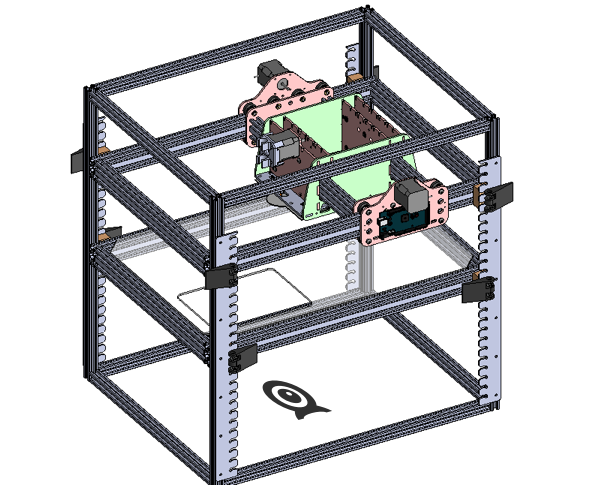
\includegraphics[width=0.48\textwidth]{immagini/observational-layer.png}
\end{center}
	 \caption{La struttura completa del robot}
	\end{wrapfigure} 
Il robot, come schematizzato in Figura 1, è composto da tre strati: dal basso si ha lo strato dell'\emph{osservazione}, all'interno del quale è posta una webcam statica utilizzata sia per la registrazione degli esperimenti, sia per l'interazione con il robot. Il secondo strato, degli \emph{esperimenti}, è composto da una superficie di vetro trasparente sulla quale vengono sistemati i recipienti richiesti dagli specifici esperimenti. L'ultimo strato, lo strato dell'\emph{attuazione} è composto dalla testa del robot. Questa struttura si muove a livello orizzontale lungo il piano. La testa è composta da circuiti stampati costituiti da connettori a molla per l'inserimento di moduli specifici. Ad oggi esiste soltanto il modulo siringa ma si prevede nel breve futuro, la costruzione di altri moduli come sensori di pH e di temperatura. 
\\Il modulo siringa ha due gradi di movimento verticale. Ogni modulo è composto di un motore passo-passo lineare per il movimento dello stantuffo, \emph{plunger}, e di un meccanismo a rocchetto e cremagliera con un secondo motore passo-passo per il movimento del corpo della siringa. La siringa può essere facilmente sostituita dando all'utente l'opportunità di utilizzare siringhe con specifiche differenti in base alle necessità del singolo esperimento. Le siringhe sono la componente di EvoBot che gli permette la gestione di sostanze liquide. 
\\Il robot può essere controllato manualmente o con programmi appositamente sviluppati con le API messe a disposizione da EvoBot. Per controllare manualmente EvoBot si utilizza Printrun \cite{printrun}, una \emph{3D printing host suite}  opensource, con la quale, attraverso dei codici G standard, si controlla il movimento della testa del robot e con dei codici M speciali si controlla il movimento delle siringhe e degli stantuffi.

\textbf{L'esperimento}
\begin{wraptable}{r}{0.5\textwidth}
\caption{Spazio multiparametrico degli esperimenti}
\begin{center}
\begin{tabular}{l|l|l|l}
\backslashbox{\textbf{molarità}}{\textbf{ph}} & \textbf{11} & \textbf{12} & \textbf{13} \\ \hline
\textbf{20mM} &  &   &   \\ \hline
\textbf{10mM} &    &   &   \\ \hline
\textbf{5mM}  &    &  &  \\ \hline
\end{tabular}
\end{center}
\end{wraptable}
Una delle proprietà fondamentali degli organismi viventi è l'abilità di sentire e rispondere ai cambiamenti dell'ambiente tramite il movimento. 
Una cellula che percepisce delle molecole solubili può muoversi lungo il gradiente di concentrazione creato da queste fino a raggiungere la sorgente oppure allontanarsi da questa nel caso in cui le sostanze rilasciate siano repellenti o tossine.
Il movimento preso in analisi è un movimento di \emph{chemiotassi}. La \emph{chemiotassi} può essere di tipo positivo in caso di avvicinamento alla sorgente e di tipo negativo in caso di allontanamento. Lo studio è stato svolto sul movimento chemiotattico positivo promosso da una \emph{droplet} di decanolo in soluzione acquosa di Acido decanoico $(CH_{3}(CH_{2})_8COOH)$ lungo il gradiente di concentrazione creato dall'aggiunta di Cloruro di sodio. Il movimento di auto-avanzamento di oggetti non biologici simula il comportamento chemiotattico di cellule viventi. 
\\Una \emph{droplet} posizionata sulla superficie di un substrato, può muoversi quando la superficie sottostante cambia il proprio motivo in modo asimmetrico creando una differenza nella tensione interfacciale tra il margine anteriore e il margine posteriore della droplet. 
Inoltre una \emph{droplet} può rompere la simmetria attraverso una reazione chimica accoppiata che avviene all'interfaccia tra la droplet e la soluzione circostante. La reazione chimica produce una rottura della simmetria dovuta all'accumulo e al rilascio di prodotti che inducono la droplet a muoversi attraverso la soluzione acquosa.\cite{selfpropelled}
\\In particolare, e' stata analizzata la dipendenza parametrica della risposta chemiotattica della droplet al variare della concentrazione e del pH di Sodio Decanoato in rapporto alla forza del gradiente di concentrazione di $NaCl$ $3.5M$. 
Lo spazio multiparametrico utilizzato ha previsto l'esecuzione di ripetizioni di ognuno dei nove esperimenti composti come in tabella 1.

\textbf{Tecniche utilizzate}
\\Analizzando i diversi comportamenti della droplet nei vari esperimenti eseguiti e tenendo in considerazione che l'obiettivo di tale studio è quello di fare in modo che questa si muova velocemente e in maniera precisa lungo un percorso ipotizzato, si è cercata la combinazione ``migliore" dei parametri sperimentali che permettesse alla droplet di avvicinarsi il più possibile e nel minor tempo al punto in cui il sale è stato posto. 
\begin{wrapfigure}{r}{0.5\textwidth}
\begin{center}
	  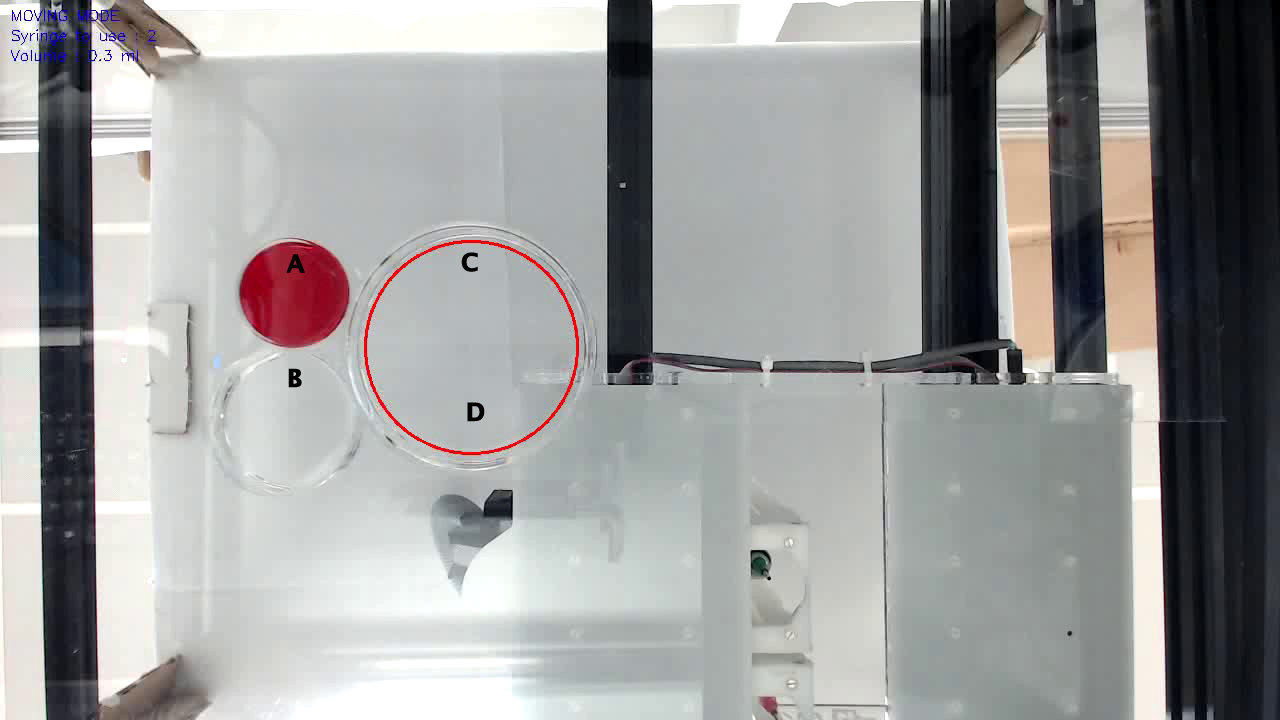
\includegraphics[width=0.3\textwidth]{immagini/exp1.jpg}
\end{center}
	 \caption{Disposizione dell'esperimento}
\end{wrapfigure} 
Lo studio di questo movimento di chemiotassi, ci aiuterà a comprendere e a riprodurre le dinamiche di movimento delle cellule viventi. 
L'esperimento precedentemente descritto, è stato eseguito per mezzo del programma appositamente sviluppato, utilizzando le API di EvoBot e sfruttando funzioni avanzate della libreria OpenCV. 
Per portare a termine l'intero esperimento occorre completare tre fasi: preparazione, raccolta dati ed elaborazione dati. 
Nella preparazione si utilizza la disposizione come in Figura 2 e un protocollo caratterizzato dai seguenti passaggi fondamentali:
\\1. Limitazione dell'area di interesse: attraverso l’apposita interfaccia è possibile disegnare un cerchio attorno alla Petri dish, permettendo così di non considerare tutto ciò che si trova all'esterno di questo limite virtuale dal programma.
\\2. Gestione del decanolo: prelevare $50\mu L$ di decanolo utilizzando una siringa delle due a disposizione, si raggiunge il pozzetto A e si fa scendere il corpo della siringa per prelevare la quantità di decanolo richiesta. Rilasciare $30\mu L$ di decanolo posizionando la siringa precedentemente caricata sopra la Petri dish in posizione C, si rilascia il decanolo. 
\\3. Gestione del sale: prelevare $500\mu L$ di NaCl utilizzando l'altra siringa, si raggiunge il pozzetto B e si eseguono le stesse azioni del punto 2, prelevando questa volta il sale. Immettere $200\mu L$ di NaCl posizionando la siringa attualmente in uso sopra la Petri dish in posizione D, si rilascia il sale. 
\\Tramite l'utilizzo della webcam statica e la libreria di OpenCV, il programma permette di tracciare passo-passo i movimenti della droplet, fino a 30 al secondo. \\Nel nostro caso ci siamo soffermati ad osservare se ci fosse un movimento della droplet verso il sale e si è cercato di capire in che ambiente questo risultasse più veloce e più preciso. Nella raccolta dei dati il programma si serve del salvataggio di questi su di un file \emph{.csv}. Un esempio di questo file è disponibile nella tabella sottostante. 
\begin{center}
\begin{tabular}{lllllll}
X salt & Y salt & X droplet Start & Y droplet Start & X droplet End & Y droplet End & time(s) \\
\hline
405    & 418    & 378             & 300             & 425           & 434           & 88  
\end{tabular}
\end{center}
I file prodotti durante la raccolta dati, vengono successivamente presi in carico da un altro programma che ha il compito di analizzare queste rilevazioni col fine di generare un unico file contenente dati e metadati dei singoli esperimenti. La colonna più importante del file generato è quella che prende il nome di ``k". Questo coefficiente indica la precisione con cui la droplet si avvicina al sale ed è definita come:
\begin{equation} 	
	k := \frac { d(C,B) }{ d(A,C) }
\end{equation}
Dove A rappresenta il punto in cui la droplet viene trovata all'inizio del tracking, B quello in cui viene posizionato il sale, C dove la droplet si trova ad esperimento concluso, ed infine $d$ calcola la distanza euclidea tra i punti in questione. 
\\Possiamo assumere che più $d(C,B)$ tende a zero, più l'esperimento è preciso; da questo si evince che avere un $k$ tendente a zero è indice di successo. Una volta ottenuti tutti i $k$, mantenendo costante il $pH$ e le molarità, si vanno a calcolare tutti i $k$ medio per ogni singolo ambiente. L'ambiente rappresentato dal minor $k$ medio è quello che permette alla droplet di raggiungere il sale in maniera precisa e veloce. \\

\textbf{Risultati raggiunti}
\\I dati hanno dimostrato che nelle soluzioni $10mM$ e $5mM$ la droplet compie dei percorsi più lunghi, arrivando molto vicina al punto di inserimento del sale. Tuttavia, nelle soluzioni $20mM$ si osservano dei movimenti più brevi, come se la droplet facesse fatica a riconoscere il gradiente del sale compiendo un movimento minimo. Bisogna tenere in considerazione che questo movimento può essere influenzato da flussi di aria capaci di creare dei moti convettivi all'interno del sistema. I moti possono agire come forza contraria alla direzione del movimento. 
\begin{wraptable}{r}{0.55\textwidth}
\caption{Tabella riassuntiva}
%\begin{center}
\begin{tabular}{l|lll}
\backslashbox{\textbf{molarità}}{\textbf{ph}} & \textbf{11} & \textbf{12} & \textbf{13} \\ \cline{1-4} 
\textbf{20mM} & 2,013 & 3,357 & 4,742 \\ 
\textbf{10mM} & 0,373  & 0,504 & 0,592 \\ \cline{2-2}
\multicolumn{1}{l|}{\textbf{5mM}} & \multicolumn{1}{l|}{0,209} & 0,67  & 0,327 \\ \cline{2-2}
\end{tabular}
%\end{center}
\end{wraptable}
\\Tuttavia queste ipotesi potranno essere confermate attraverso la ripetizione di un maggior numero di esperimenti.
Nella tabella riassuntiva 2 sono stati raccolti tutti i valori medi di ogni combinazione. Come si può osservare il coefficiente di precisione migliore si ha nella soluzione $5mM$ con $pH11$. Inoltre, le soluzioni $20mM$ hanno i coefficienti maggiori tra tutte, sinonimo di una minore precisione della droplet nel raggiungimento della sorgente di sale.





















   	
%%%%%%%%%%%%%%%%%%%%%%%%%%%%%%%%%%%%%%%%%%%%%%%%%%%%%%%%%%%%%%%%%%%%%%%%%%
%% Nota
%% Sommario e' un breve riassunto del lavoro svolto dove si descrive l’obiettivo, l’oggetto della tesi, le metodologie e le tecniche usate, i dati elaborati e la spiegazione delle conclusioni alle quali siete arrivati. Il sommario dell’elaborato consiste al massimo di 3 pagine e deve contenere le seguenti informazioni: 
%% contesto e motivazioni
%%   breve riassunto del problema affrontato
%%   tecniche utilizzate e/o sviluppate
%%   risultati raggiunti, sottolineando il contributo personale del laureando/a
%%%%%%%%%%%%%%%%%%%%%%%%%%%%%%%%%%%%%%%%%%%%%%%%%%%%%%%%%%%%%%%%%%%%%%%%%%      
      
      % lista dei capitoli
      %
      % \input oppure \include
      %
      \chapter{Introduzione}
\vspace{0.5cm}

\label{cha:intro}
\epigraph{“Why is it less acceptable to seek how to make a cell than how to make a molecule?"}{--- \textup{Stéphane Leduc}}

"Come è iniziata la vita?": la domanda più interessante che l'umanità si sia mai posta. La necessità di trovare una spiegazione al fenomeno dell'origine della vita ha portato il mondo della ricerca a soffermarsi sulla possibile riproducibilità in laboratorio di aspetti semplici degli organismi viventi. 
Nel 1911 Stéphane Leduc, biologo francese, scrisse: «[...] la sintesi della vita deve avvenire nella produzione di forme intermedie tra il mondo organico ed il mondo inorganico, forme che possiedono soltanto alcuni rudimentali attributi di vita, alle quali altri attributi verranno aggiunti nel corso dello sviluppo dall'azione dell'ambiente circostante». Questa unione di elementi provenienti dal mondo vivente e dal mondo "non vivente" ci permettere di iniziare la costruzione di strutture semplici per poi svilupparle in forme sempre più simili ad "esseri viventi". 
Lo studio affrontato in questo progetto si avvale delle tecniche della la biologia sintetica per tentare di riprodurre comportamenti molto semplici, il movimento nel nostro caso, di ciò che potrà diventare un "essere vivente" sintetizzato in laboratorio.

\section{La Biologia Sintetica}
\label{sec:artificial}
Nel 1912 appare per la prima volta il termine "biologia sintetica" coniato dal biologo francese Stéphane Leduc (1853-1939) nel libro "La Biologie Syntetique". Egli affermò: «Quando avremo modo di conoscere il meccanismo fisico della produzione di un oggetto o di un fenomeno,[...] diventa possibile[...] riprodurre l'oggetto o il fenomeno, in quel momento la scienza è diventata sintetica. La biologia è una scienza come le altre, [...] deve essere in successione: descrittiva, analitica e sintetica». 
Lo scopo del nostro progetto è  quello di riprodurre caratteristiche base degli organismi viventi, nello specifico ci si è soffermati sul movimento in un sistema chimico.
\\Il termine viene successivamente ripreso nel 1974 dal genetista polacco Wacław Szybalski: «Discutiamo ora del seguente problema, ovvero cosa avverrà dopo? Fino ad ora abbiamo lavorato sulla fase descrittiva della biologia molecolare. Ma la vera sfida partirà quando entreremo nella fase della sintesi biologica[...]. Io non credo che esauriremo idee nuove ed eccitanti[...] nella biologia sintetica.» \cite{waclaw} 
\\Al fine di "sintetizzare" un essere vivente, le caratteristiche da ricercare sono:
\begin{itemize}
\item un corpo: per distingue il soggetto dall'ambiente circostante
\item un metabolismo: processo per il quale il soggetto prende risorse dall'ambiente e le trasforma in sostanze di mantenimento
\item informazione ereditabile: contenuta nel genoma ed in grado di essere passata alle generazioni successive
\end{itemize}
L'unione dei primi due punti ci porta ad avere un organismo in grado di muoversi e replicarsi, se in seguito aggiungessimo la capacità di passare l'informazione genomica avremmo così realizzato un soggetto evolutivo.
La Biologia Sintetica prevede due approcci diversi, nel primo caso si cerca di ricreare una nuova funzione e applicazione riprogrammando organismi già esistenti. Il secondo approccio prevede la sintesi da zero di forme di vita artificiale con alcune funzionalità degli esseri viventi aggiungendo singoli componenti al sistema. Il progetto si è focalizzato su questo approccio. Varie sostanze chimiche vengono utilizzate e riorganizzate in strutture e reti che si comportano come sistemi viventi. I sistemi vengono alimentati con opportuni nutrienti e viene osservato il loro comportamento, nello specifico il movimento, altra caratteristica fondamentale di un organismo vivente.
\pagebreak
\section{Il progetto EVOBLISS}
\label{sec:context}
Il progetto EVOBLISS  è un progetto di ricerca europeo finanziato dalla Commissione Europea FET (Future and Emerging Technologies). A questo progetto partecipano i laboratori di cinque diverse università europee:
\begin{itemize}
\item IT University of Copenhagen (ITU) – Denmark
\item University of West of England (UWE) – Bristol, Great Britain
\item Karlsruhe Institute of Technology (KIT) – Germany
\item University of Glasgow (UGL) – Great Britain
\item Università degli Studi di Trento – Italy
\end{itemize}
Il progetto mira a sviluppare un tipo di evoluzione artificiale e tecnologica da utilizzare per la progettazione di sistemi funzionali composti da tre forme di \emph{living technology}: vita chimica artificiale, microrganismi viventi e da reti di reazioni chimiche complesse usate per migliorare il processamento e la purificazione di acque di scarico per la generazione di energia.
Il progetto EVOBLISS combina gli approcci scientifici della robotica, dell'intelligenza artificiale, della chimica e della microbiologia per sfruttare al meglio le avanguardie di queste discipline. Lo scopo finale è quello di produrre una piattaforma robotica facilmente utilizzabile e personalizzabile per l'evoluzione artificiale di nuovi materiali e per l'ottimizzazione delle performance di sistemi psicochimici e microbici. Il prodotto su cui si è lavorato è EvoBot, un robot in grado di gestire liquidi e di fornire riscontri in tempo reale. 

\subsection{EVOBLISS a Trento}
\label{sec:trento}
Il laboratorio di Biologia Artificiale del CIBIO - Centre for Integrative Biology dell'Università di Trento è parte integrante del progetto EVOBLISS.
Qui ci si occupa di sviluppare diversi tipi di cellule artificiali basandosi su emulsioni \emph{droplet-based}. 
Le \emph{droplets} a cui si fa riferimento sono composte da \emph{1-Decanolo} $(C_{10}H_{21}OH)$. Il decanolo è formato da una catena lineare di alcol grasso con 10 atomi di carbonio.\cite{decanolo} Essendo incolore vi si aggiunge \emph{Oil Red O} \cite{oilredo}, un colorante solubile con i grassi che lo rende visibile all'occhio umano e ci permette di tenerne traccia all'interno del sistema. Le \emph{droplets} analizzate hanno volume pari a $30\mu l$, il volume è stato scelto per avere una migliore  tracciabilità dal programma di analisi di \emph{computer vision}.
Le caratteristiche prese in analisi sono simili a quelle che possono caratterizzare un essere vivente: l'auto-movimento, l'auto-divisione, la trasformazione biochimica e le dinamiche di gruppo.
\\La piattaforma è stata qui adattata alla necessità di monitorare il movimento delle \emph{droplets} a partire dal momento in cui queste escono da un sistema di equilibrio, studiando l'ottimizzazione dei parametri che definiscono l'ambiente in cui queste si muovono. Lo scopo ultimo è quello di incrementare la conoscenza delle \emph{living technologies} e di ideare e sfruttare al meglio sistemi bio-ibridi innovativi.
Ulteriori studi hanno visto l'implementazione di programmi per il riconoscimento di droplets multiple. 
 
















      \chapter{La piattaforma robot}
%\vspace{0.5cm}

\label{cha:789}
EvoBot è un robot che unisce elementi delle stampanti 3D con quelli della robotica modulare per fornire a chimici, microbiologi e ricercatori nel campo della vita (a livello chimico) artificiale, uno strumento economico ed estendibile basato su una piattaforma open source di robotica per il trattamento di liquidi. La particolarità di EvoBot sta nell'interazione continua ed in tempo reale dell'utente con l'esperimento in corso.\cite{introd-robot} Inoltre utilizzare un robot per la gestione degli esperimenti ci ha permesso di diminuire, quasi annullare, l'incertezza e la variazione tra gli esperimenti causata dalla mano umana. 
\\Come le comuni stampanti 3D,  questo robot è composto da una componente hardware guidata da una parte software. 

\section{La componente hardware}
EvoBot è composto, a livello elettronico, da un Arduino Mega 2560 su cui è montata una scheda RAMPS (RepRap Arduino Mega Pololu Shield); queste due schede controllano la testa del robot, i moduli ad essa collegati e gli input provenienti da sensori esterni. 
A livello meccanico, invece, è strutturato in tre strati: \emph{actuation layer}, \emph{experimental layer} e  \emph{observation layer}.
\\Partendo dal basso si trova lo strato dell'osservazione: \emph{observation layer}. Questo \emph{layer} non prevede nessuna interazione con gli esperimenti in corso sul layer superiore. E' utilizzato per il posizionamento di moduli che andranno a raccogliere dati, senza manipolare direttamente l'esperimento, che verranno forniti sia al robot sia all'utente. Nel nostro caso è presente una webcam. 
	\begin{figure}[h]
	  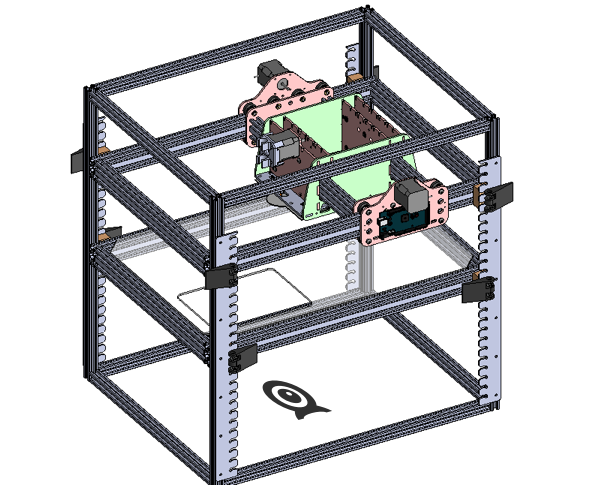
\includegraphics[scale=0.40]{immagini/observational-layer.png}
	\centering
	 \caption{La struttura completa con l'observational layer}
	\end{figure} 

\pagebreak
Il secondo strato è quello degli esperimenti: \emph{experimental layer}. Questo strato è essenzialmente composto da una cornice in alluminio, identica a quella della struttura esterna del robot, che racchiude una piastra di vetro. Su questo strato possono essere posti i recipienti richiesti dagli specifici esperimenti. Una fessura rettangolare ad uno degli angoli permette le manovre di sostituzione dei recipienti in uso. La sua funzionalità verrà sfruttata in futuro creando un distributore automatico di  \emph{Petri dish} da posizionarvi all'interno.
	\begin{figure}[h]
	  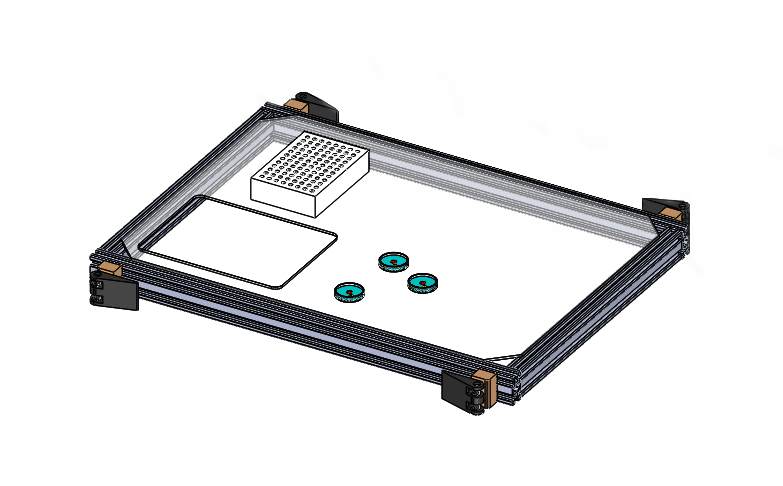
\includegraphics[scale=0.40]{immagini/experiment_layer.png}
		\centering 
	\caption{experimental layer}
	\end{figure} 
\\L'ultimo dei tre strati è lo strato di attivazione, \emph{actuation layer}, ovvero la testa del robot.  Questo layer si occupa del movimento della testa sul piano orizzontale per mezzo di un meccanismo cinghia-ruota dentata con due motori \emph{stepper}. La testa si può muovere nelle due direzioni sul livello orizzontale: \emph{x} e \emph{z}.

	\begin{figure}[h]
	  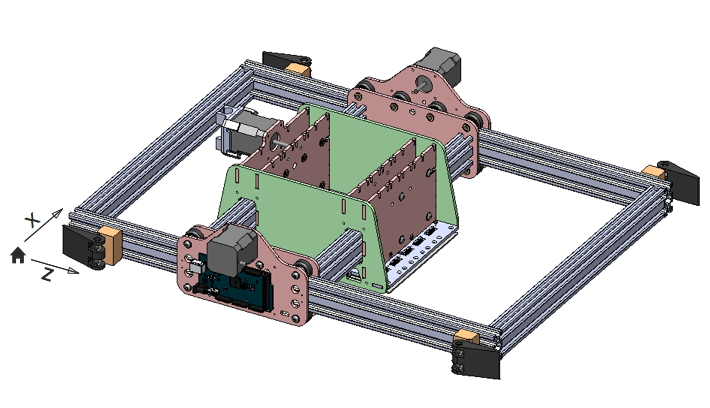
\includegraphics[scale=0.30]{immagini/actuation_layer.png}
		\centering	
	 \caption{actuation layer}
	\end{figure}
\pagebreak

\subsection{La testa}
La \emph{head}, testa del robot, è la componente principale dell'\emph{actuation layer}. E' composta di 17 \emph{socket} all'interno delle quali possono essere inseriti diversi moduli. Tuttavia, per come è stata strutturata, non c'è possibilità di inserire tutti i moduli contemporaneamente. Essa può contenere fino ad un massimo di 11 moduli per fornire funzionalità differenti. Ad oggi esiste soltanto il modulo siringa ma si prevede nel breve futuro, la costruzione di altri moduli come sensori di pH e di temperatura. 
	\begin{figure}[h]
	\centering
   		{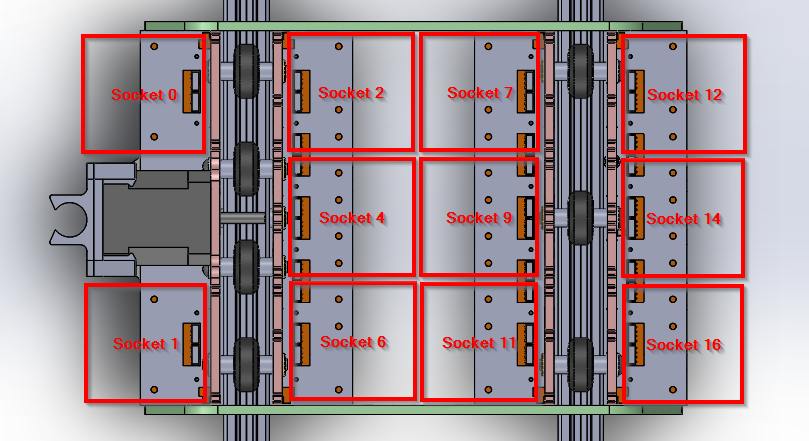
\includegraphics[width=8cm]{immagini/head_sockets_1.png}}
 	\hspace{5mm}
   		{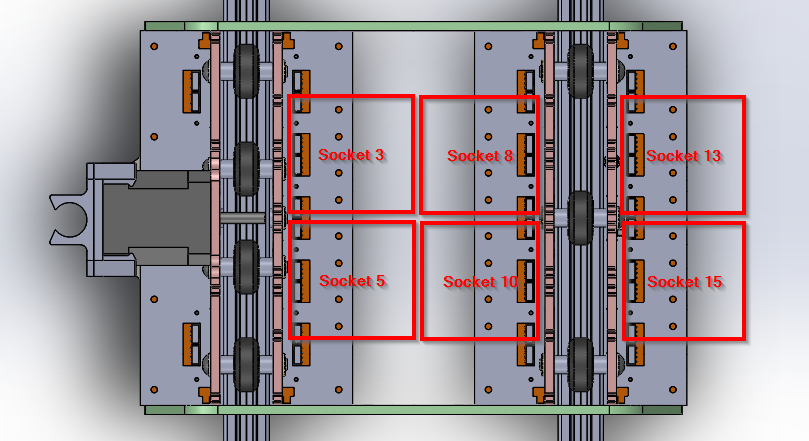
\includegraphics[width=8cm]{immagini/head_sockets.png}}
	\caption{socket disposition}
 	\end{figure}


\subsection{Le siringhe}
\label{sec:01456}
Il modulo siringa ha due gradi di movimento verticale. Ogni modulo è composto di un motore passo-passo lineare per il movimento dello stantuffo, \emph{plunger}, e di un meccanismo a rocchetto e cremagliera con un secondo motore passo-passo per il movimento del corpo della siringa. La siringa può essere facilmente sostituita dando all'utente l'opportunità di utilizzare siringhe con specifiche differenti in base alle necessità dell'esperimento. Le siringhe sono la componente di EvoBot che gli consente di gestire sostanze liquide.
	\begin{figure}[h]
	  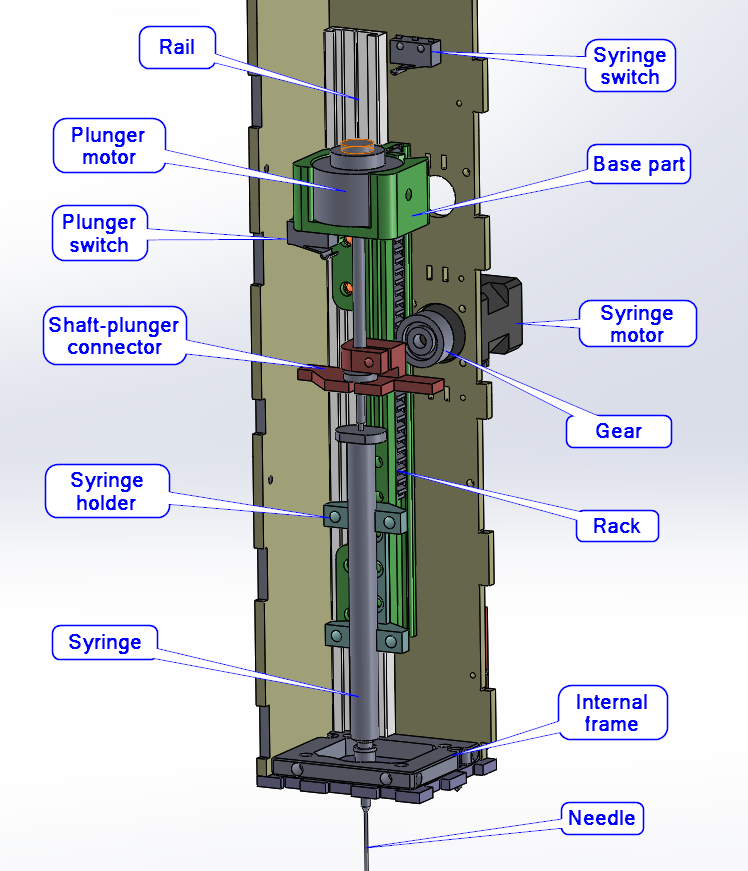
\includegraphics[scale=0.30]{immagini/syringe_parts.png}
		\centering
	 \caption{syringe module}
	\end{figure} 

\pagebreak 
\section{La componente software}
\label{sec:123}
La finalità della componente software è quella di fornire all'utente finale un'interfaccia facilmente programmabile per guidare il robot. Il software è suddiviso in una \emph{host side} e in una \emph{robot side}. La prima comunica con la seconda attraverso una connessione USB. La \emph{robot side} è una versione modificata del firmware Marlin usato nei programmi opensource delle stampanti 3D. 
\\Il linguaggio di programmazione utilizzato per la stesura delle API e dei programmi successivi è Python. La suite software offerta al momento dell'installazione è composta da tre elementi:
un programma di \emph{computer vision} per la calibrazione del robot, un'interfaccia grafica per il controllo manuale del robot ed un esempio di programma, sviluppato utilizzando le API, per l'identificazione delle componenti di uno specifico esperimento.
\\L'obiettivo dello sviluppo della componente software è stato quello di creare un programma in grado di controllare il robot manualmente in tempo reale e raccogliere i dati necessari dagli esperimenti eseguiti, di cui si parlerà nel prossimo capitolo. 

\subsection{Il controllo manuale}
\label{sec:00123}
La scelta di un software per il controllo manuale del robot nasce dalla necessità di ottenere la posizione di oggetti di interesse (Petri dishes e recipienti vari) sullo strato degli esperimenti. L'interfaccia grafica permette di testare le diverse funzioni del robot senza il bisogno di ricorrere alla programmazione. Per esempio, si può muovere la testa del robot fino a centrare uno dei contenitori, far scendere la siringa all'interno di questo e registrare la posizione del centroide dell'oggetto. 
\\Per controllare manualmente EvoBot si utilizza Printrun \cite{printrun}, una \emph{3D printing host suite}  opensource, con la quale, attraverso dei codici G standard, si controlla il movimento della testa del robot e con dei codici M speciali si controlla il movimento delle siringhe e degli stantuffi. Inoltre con i codici M si possono identificare i limiti dei due movimenti che una siringa può compiere.

\subsection{La calibrazione}
\label{sec:01123}
La calibrazione è il primo passo importante per correlare il sistema di coordinate della videocamera con quello del robot. A questo scopo viene creata la matrice di trasformazione compiendo le istruzioni imposte dal programma calibrationExample.py. 
Avendo la possibilità di posizionare le differenti piastre di Petri su tutto lo strato degli esperimenti o di impostare la distanza tra \emph{l'actuation layer} e \emph{experimental layer}, il programma è pensato per specificare i punti esatti per una massima accuratezza nella calibrazione. All'interno del programma si definisce il punto in cui è posizionata la Petri \emph{dish}, il suo diametro e la distanza tra i due layer.
Avvenuta la calibrazione, si hanno a disposizione le matrici di ogni siringa da poter utilizzare nei programmi successivi per muovere le siringhe nei punti richiesti dagli esperimenti.

\subsection{L'identificazione delle \emph{droplets}}
\label{sec:02123}
Una delle finalità prioritarie del progetto è l'identificazione di gocce, \emph{droplets}, per trovare l'area, il colore, il numero, la forma e, più importante, per tracciarne il movimento.
%Come spiegato nella sezione 1.2.1le droplet.... aggiungere minchiate

La componente principale utilizzata per l'identificazione è la libreria OpenCV (Open Source Computer Vision Library)\cite{opencv} che include diverse funzioni ed algoritmi di \emph{computer vision}. 











 


      \chapter{Il sistema chimico}
\vspace{0.5cm}
\label{cha:789}

Una delle proprietà fondamentali degli organismi viventi è l'abilità di sentire e rispondere ai cambiamenti dell'ambiente tramite il movimento. 
Se consideriamo la cellula, in termini generali, come un sistema chimico aperto in una situazione di non-equilibrio, è essenziale avere a disposizione un rifornimento di materiale fresco e di energia per sostenerla. Per fare in modo che questo avvenga, la cellula modifica il suo ambiente esterno metabolizzando risorse di sostentamento e producendo dei prodotti e degli scarti. Per evitare una situazione statica, di equilibrio, il sistema deve trovare in qualche modo nuove risorse ed evitare possibili effetti inibitori dei prodotti di scarto. In questo senso puramente chimico-biologico si crede che l'abilità di movimento giochi un ruolo importante per evitare lo stato di equilibrio nella creazione di sistemi cellulari artificiali. \cite{doi:10.1021/ja0706955}

\section{Chemiotassi e Chemiochinesi}
\label{sec:456}
Le cellule sono in grado di avvertire molecole solubili presenti nell'ambiente esterno ad esse e di percepirne eventuali cambiamenti; sono ad esempio capaci di percepire la formazione di gradienti di concentrazione. 
Una cellula che percepisce delle molecole solubili può muoversi lungo il gradiente di concentrazione creato da queste fino a raggiungere la sorgente oppure allontanarsi da questa nel caso in cui le sostanze rilasciate siano repellenti o tossine.
In generale, la motilità di una cellula può essere di tre tipi:
\begin{enumerate}
\item motilità basale casuale: avviene in assenza di stimoli chimici,
\item Chemiochinesi: corrisponde ad un movimento casuale crescente, in risposta a stimoli chimici,
\item Chemiotassi: migrazione stimolata direzionale verso un gradiente chimico.
\end{enumerate}
La \emph{chemiotassi} può essere di tipo positivo in caso di avvicinamento alla sorgente e di tipo negativo in caso di allontanamento.
	\begin{figure}[h]
	  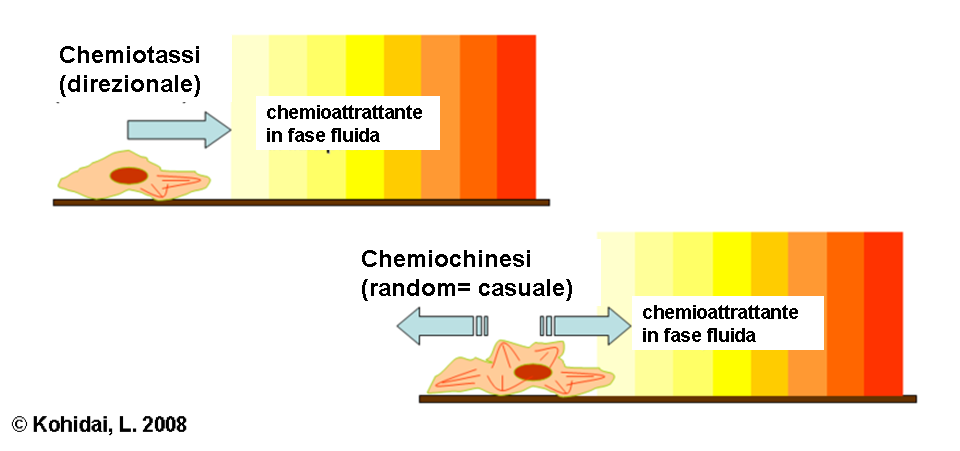
\includegraphics[scale=0.50]{immagini/chemochin.png}
		\centering	
	 \caption{chemiotassi e chemiochinesi}
	\end{figure}
\pagebreak
\\E' stato qui considerato il movimento chemiotattico positivo promosso da una \emph{droplet} di decanolo in acido decanoico lungo il gradiente di concentrazione creato dall'aggiunta di Cloruro di sodio.

\subsection{L'importanza del movimento}
\label{sec:00456}
Per gli organismi multicellulari la chemiotassi è importante nei processi fisiologici, come il reclutamento di cellule del sistema immunitario nei siti dell'infezione e negli organi dello sviluppo durante l'embriogenesi.\cite{cellMig} Le cellule neuronali e quelle embrionali, invece, migrano durante lo sviluppo. Durante l'angiogenesi, le cellule endoteliali vanno incontro a chemiotassi per formare i vasi sanguigni, mentre le cellule epiteliali e i fibroblasti si muovono con chemiotassi durante la guarigione di una ferita.\cite{move1} Tuttavia, oltre al ruolo in processi ovviamente benefici, la chemiotassi è coinvolta anche in tutti gli stadi cruciali del tumore cellulare, dalla disseminazione alla progressione delle metestasi. Molte cellule cancerogene, nello specifico quelle del tumore al seno, sono note per avere la preferenza nel metastatizzarsi in specifici organi e tessuti. Questa preferenza è correlata alla produzione di chemioattraenti del tessuto e degli organi bersaglio e ad una sovrapproduzione dei recettori di queste sostanze sulla superficie delle cellule cancerose \cite{chemocancer}.
Il movimento spontaneo di \emph{droplets} liquide, particelle solide e gel in condizioni di non-equilibrio, è stato spesso studiato sia a livello teorico che sperimentale. Il movimento di auto-avanzamento di oggetti non biologici può simulare il comportamento chemiotattico o chemiocinetico di cellule viventi.
Come nel caso di organelli mobili e cellule che esibiscono polarità, è necessaria una rottura spontanea della simmetria per scatenare l'auto-movimento di oggetti non-biologici. 
\\Una \emph{droplet} posizionata sulla superficie di un substrato, può muoversi quando la superficie sottostante cambia il proprio motivo in modo asimmetrico creando una differenza nella tensione interfacciale tra il margine anteriore e il margine posteriore della droplet. Inoltre una \emph{droplet} può rompere la simmetria attraverso una reazione chimica accoppiata che avviene all'interfaccia tra la droplet e la soluzione circostante. La reazione chimica produce una rottura della simmetria dovuta all'accumulo e al rilascio di prodotti che inducono la droplet a muoversi attraverso la soluzione acquosa.\cite{selfpropelled}
\\Il motivo del percorso della droplet osservato in questo studio è di tipo rettilineo ed è stato analizzato con un software di analisi visuale. 

\section{Componenti inorganiche}
\label{sec:123}
Questo studio ha esaminato in particolare la dinamica di una \emph{droplet} di decanolo  che si muove chemiotatticamente in una soluzione acquosa di Acido decanoico $(CH_{3}(CH_{2})_8COOH)$ lungo i gradienti di concentrazione formati con l'aggiunta di Cloruro di sodio $(NaCl)$.\cite{ikea}
\\E' stata analizzata la dipendenza parametrica della risposta chemiotattica della droplet al variare della concentrazione e del pH di Sodio decanoato in rapporto alla forza del gradiente di concetrazione di $NaCl$. 
Lo spazio multiparametrico utilizzato ha previsto l'esecuzione di due ripetizioni di ognuno dei nove esperimenti così composte: 
\begin{table}[htbp] 
  \begin{center} 
    \begin{tabular}{c|cccc} 
      \textbf{molarità} & & \textbf{pH}\\ 
      \midrule 
	& 11 & 12 & 13\\ 
\hline
	5mM\\
\hline
	10mM\\
\hline
	20mM\\ 
	\hline 
     \end{tabular} 
   \end{center} 
	\caption{spazio multiparametrico degli esperimenti}
\end{table}

Le soluzioni di acido decanoico in fase acquosa sono state preparate sciogliendo $3,44gr$ di Acido decanoico  in $1L$ di acqua per avere una soluzione $20mM$. Con l'aggiunta di $10mL$ di $NaOH$ si è ottenuta una soluzione con $pH 13$. 
Da questa si sono creati gli \emph{stock}, a $pH13$, da $100mL$ ciascuno per le soluzioni nelle differenti molarità: $5mM$ diluendo $1/4$ del volume con acqua, $10mM$ diluendone $1/2$ e $20mM$ tenendo la soluzione non diluita.
\\Ulteriori $300mL$ della soluzione di partenza sono stati utilizzati per le soluzioni a $pH 12$, il livello desiderato di pH è stato raggiunto con l'aggiunta di $10\mu L$ di $HCl$. Anche di questi si sono create le diluizioni con molarità $5mM$, $10mM$ e $20mM$. 
\\I restanti $300mL$ sono stati utilizzati per le soluzioni a $pH11$ con ulteriore aggiunta di $20\mu L$ di $HCl$; applicando le stesse diluizioni per le stesse molarità.
La soluzione di $NaCl$ utilizzata è stata ottenuta disciogliendo $10,227gr$ di $NaCl$ in acqua per avere la molarità a $3,5M$.
\\Per rendere le droplets di decanolo visibili al software di analisi, si è aggiunto il colorante Oil Red O a $20mL$ di decanolo in piccola quantità, fino al completo scioglimento.  







      \chapter{Raccolta dati ed analisi}
\vspace{0.5cm}
\label{cha:789}

Tra i parametri sperimentati si è cercata la combinazione "migliore": quella che permette alla droplet di arrivare il più possibile vicino al punto in cui il sale è stato inserito nel sistema muovendosi nel minor tempo possibile. Questo è stato possibile analizzando i diversi comportamenti della droplet in ognuna delle nove combinazioni. La scelta è stata fatta tenendo in considerazione che l'obiettivo dello studio è quello di fare in modo che la droplet si muova velocemente lungo un percorso specifico e definito. Lo studio di questo movimento di chemiotassi ci aiuta a comprendere e riprodurre le dinamiche di movimento delle cellule viventi. 

\section{Il software}
Il software implementato per la raccolta dei dati è stato creato utilizzando le API della piattaforma robotica per gestire il robot e sfruttando delle funzioni avanzate della libreria OpenCV. Il robot viene controllato manualmente dall'utente che può scegliere tre modalità di azione: \emph{setting mode}, \emph{moving mode}, \emph{tracking mode}. Il passaggio fra le varie modalità è gestito rispettivamente con il click sui numeri "1" "2" e "3" sulla tastiera. La modalità in cui l'utente si trova è mostrata in alto a sinistra nella schermata video. E' possibile registrare l'esperimento in corso in qualsiasi momento facendo click sul tasto "R" della tastiera; la scritta "RECORDING" appare accanto alla dicitura della modalità in cui ci si trova. Il video verrà salvato in una cartella definita all'interno del programma.
L'interazione è possibile grazie alla semplice interfaccia grafica mostrata in figura.
\begin{figure}[h]
	\centering
   		{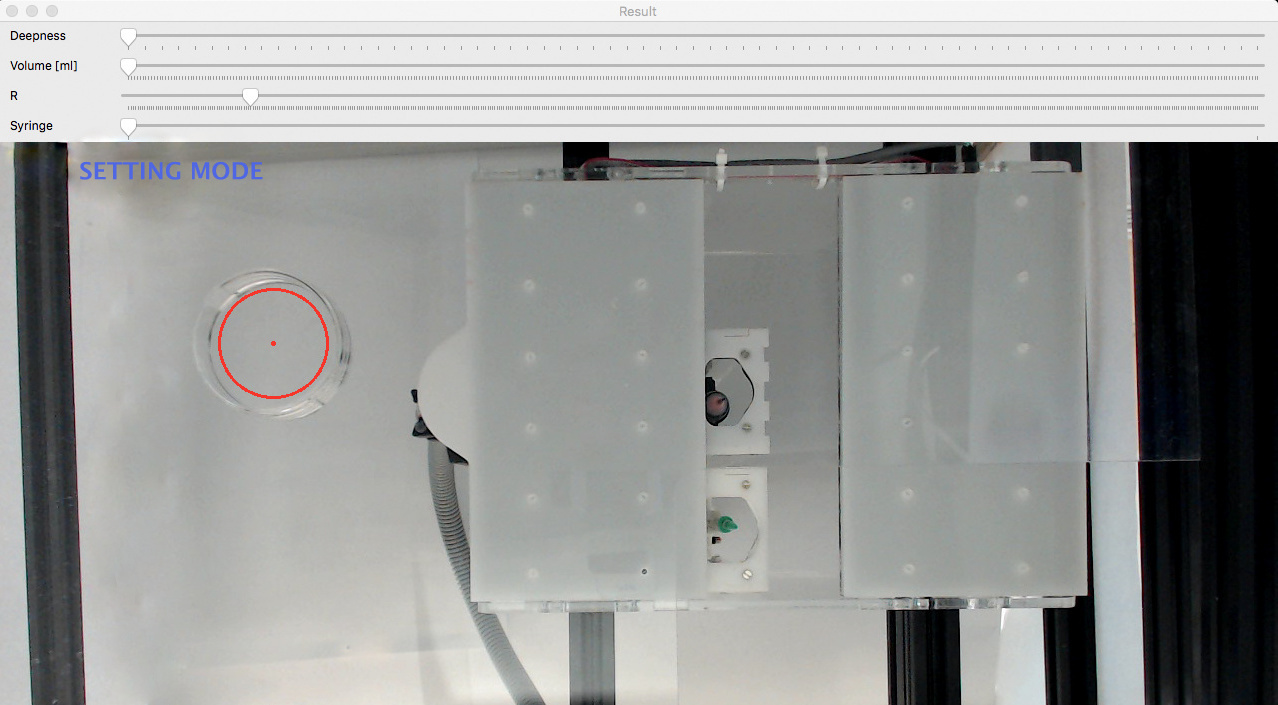
\includegraphics[width=7.5cm, height=5.5cm]{immagini/settingMOD2.jpg}}
 	\hspace{2mm}
   		{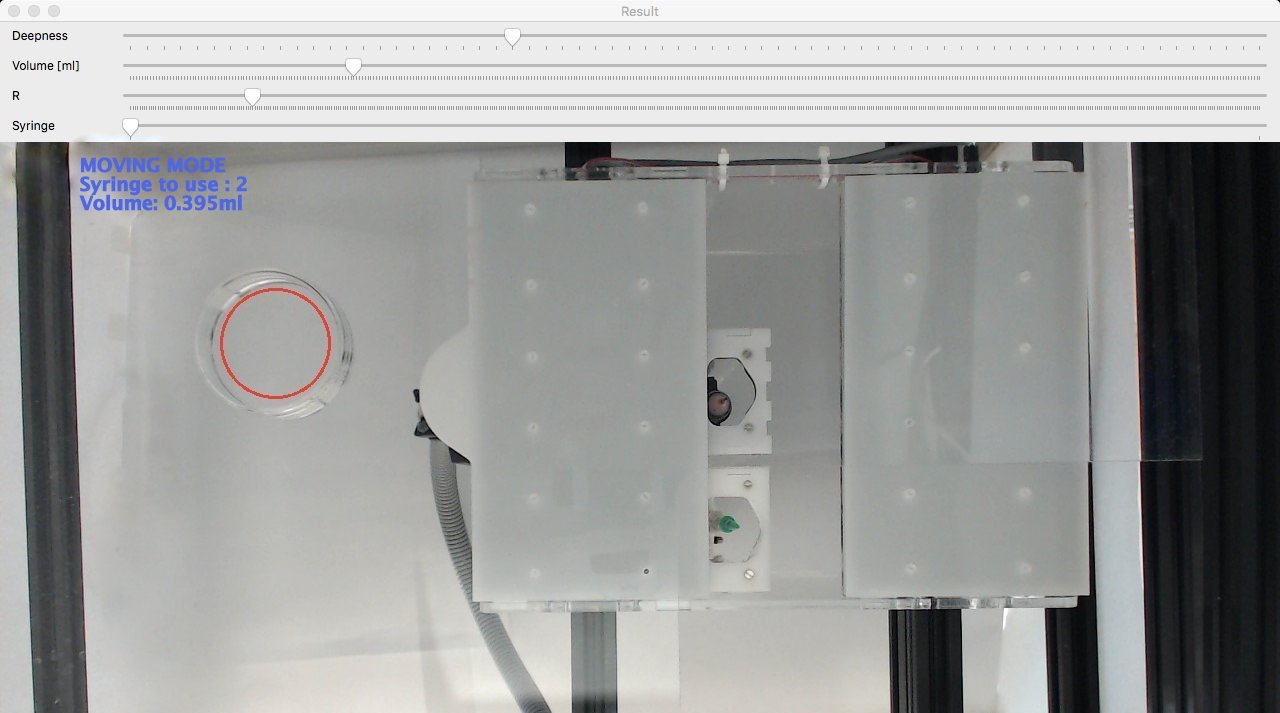
\includegraphics[width=7.5cm, height=5.5cm]{immagini/moving.jpg}}
	\caption{setting mode e moving mode}
 	\end{figure}
\\La parte superiore della finestra mostra tre barre di controllo. La prima indica la \emph{deepness} ovvero la profondità a cui il corpo della siringa deve arrivare affinché il puntale raggiunga il punto desiderato. I valori possono variare da 0 a 69, limiti di costruzione delle siringhe. Per arrivare nel punto desiderato si deve tenere in considerazione anche la lunghezza della punta della siringa per fare in modo che non vada contro il vetro. La seconda \emph{trackbar} indica il volume in $mL$ da far aspirare o rimettere alla siringa. Gli stantuffi delle siringhe utilizzate per questi esperimenti variano la loro posizione nel range da 0 a 35 perciò la \emph{trackbar} del volume è stata suddivisa in 36 porzioni, ognuna delle quali equivale a $0,14mL$. La terza \emph{trackbar} viene utilizzata nella \emph{setting mode}. Questa indica il raggio R a cui si può impostare il cerchio rosso presente in figura. Questa opzione è stata inserita per dare la possibilità di utilizzare petri dishes di diametri differenti e per annullare il rumore nel video di agenti esterni. Il cerchio rosso viene impostato per indicare l'area in cui avviene l'esperimento centrando il centro della \emph{Petri dish} ed allargando il cerchio fino ai bordi della petri stessa; questa è l'unica porzione di schermo a cui verranno applicati i filtri per la nitidezza dell'immagine, per il riconoscimento dei contorni della \emph{droplet} e per tracciarne il movimento.
La lunghezza dell'ultima \emph{trackbar} varia in base al numero di moduli siringa inseriti nella testa del robot. Con questa si può scegliere la siringa da utilizzare per una determinata azione. Quando si è nella modalità di movimento, vengono visualizzati i valori impostati nelle \emph{trackbars} in alto a sinistra nella schermata. In questa modalità l'utente può far muovere la testa del robot nei punti desiderati, spostare il corpo delle siringhe e definire i volumi di liquidi da prelevare dai pozzetti magazzino ed immettere nel sistema.  
 
\subsection{Riconoscimento della droplet}
La droplet da individuare è di colore rosso, dovuto all'aggiunta del colorante Oil Red O alla soluzione di decanolo. Tuttavia, le droplets possono essere colorate non solo con il rosso ma anche con colori scelti in base alle necessità di ogni esperimento. Per il riconoscimento di uno specifico colore si utilizza un set predefinito di tre valori che l'utente può trovare ed impostare all'interno del programma: i parametri HSV, Hue Saturation Value (tonalità, saturazione e valore). Il riconoscimento di elementi del colore impostato avviene solamente all'interno dell'area definita nella \emph{setting mode} dal cerchio rosso. 

\section{L'esperimento}
\label{sec:456}
Il protocollo seguito per i nove esperimenti prevede quattro passaggi fondamentali da eseguire nella \emph{moving mode}. 
\begin{enumerate}
\item utilizzare la siringa nella socket 2 per prelevare $50\mu L$ di decanolo dal pozzetto in posizione A
\item immettere $30\mu L$ di decanolo nella Petri Dish, contenente $9mL$ di Decanoato (Acido decanoico), in posizione C
\item  utilizzare la siringa nella socket 4 per prelevare $500\mu L$ di NaCl dal pozzetto in posizione B
\item immettere $200\mu L$ di NaCl nella Petri Dish in posizione D 
\end{enumerate}
\begin{figure}[h]
	  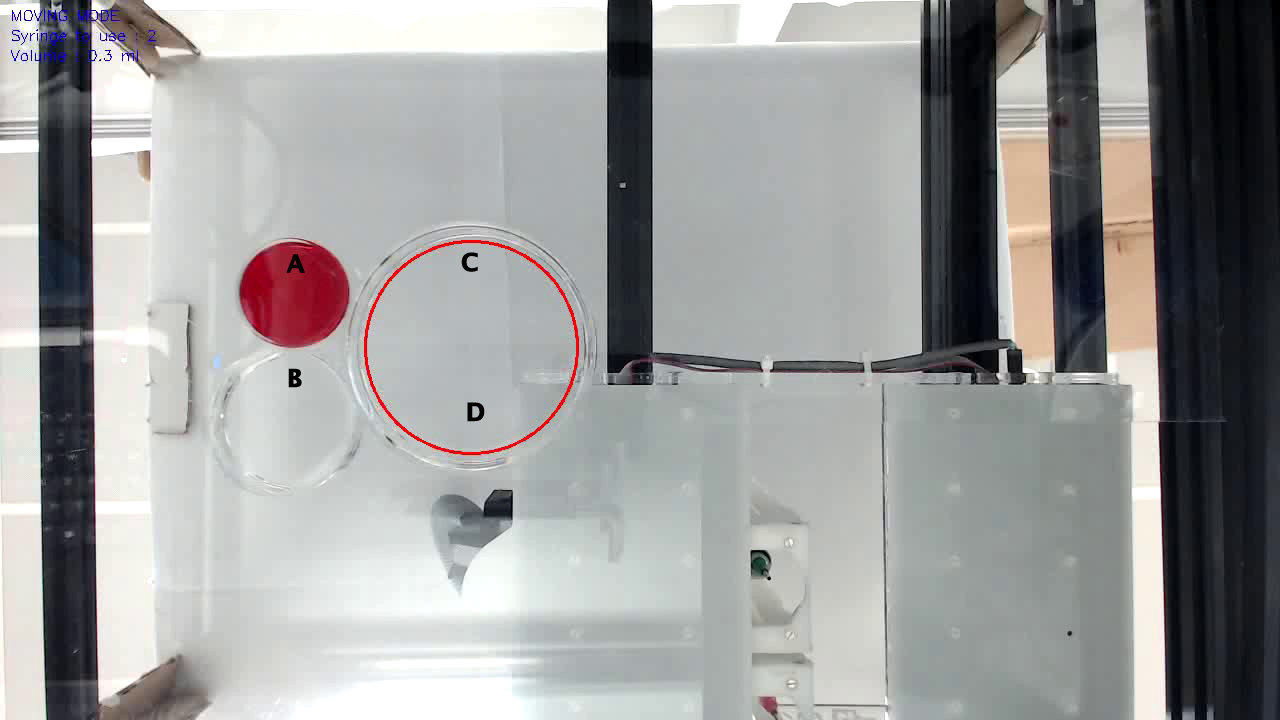
\includegraphics[scale=0.30]{immagini/exp1.jpg}
		\centering
	 \caption{experimental layout}
	\end{figure} 
La dimensione della droplet è stata definita per ottenerne una buona visibilità nella tracciabilità. 
La scelta di prelevare una quantità maggiore di liquido ci assicura l'immissione nel sistema della corretta quantità in quanto può accadere che un volume non definito venga trattenuto nel corpo o nella punta della siringa.
Le posizioni C e D all'interno della Petri sono arbitrarie e variano leggermente di esperimento in esperimento, si è cercato tuttavia, per mantenere lo spazio degli esperimenti sufficientemente uniforme, di seguire sempre lo schema proposto in figura. Questo tuttavia non è sempre stato possibile in quanto la droplet posizionata in posizione C era influenzata da moti convettivi creati dal movimento di aria attorno alla struttura del robot e dall'inserimento del puntale della siringa sulla superficie del decanoato presente nella Petri Dish. 

\subsection{Tracciabilità}
\label{sec:123}
Dopo aver posizionato la droplet di decanolo ed il sale NaCl all'interno della Petri dish, l'utente può far partire la \emph{tracking mode}. In questa modalità la testa del robot viene spostata nel punto di coordinate (0,0), in fondo a sinistra, per far in modo che non interferisca con il riconoscimento visivo. 
La droplet identificata viene circondata da un contorno verde ed indicato sulla schermata del video il colore riconosciuto. Nel momento in cui si decide di interrompere il programma, se la modalità di registrazione è attiva, appare a video il percorso eseguito dalla droplet indicante la dicitura "BEGIN" per il primo punto in cui è stata individuata, ed "END" per il punto finale di arrivo.   
\begin{figure}[h]
	\centering
   		{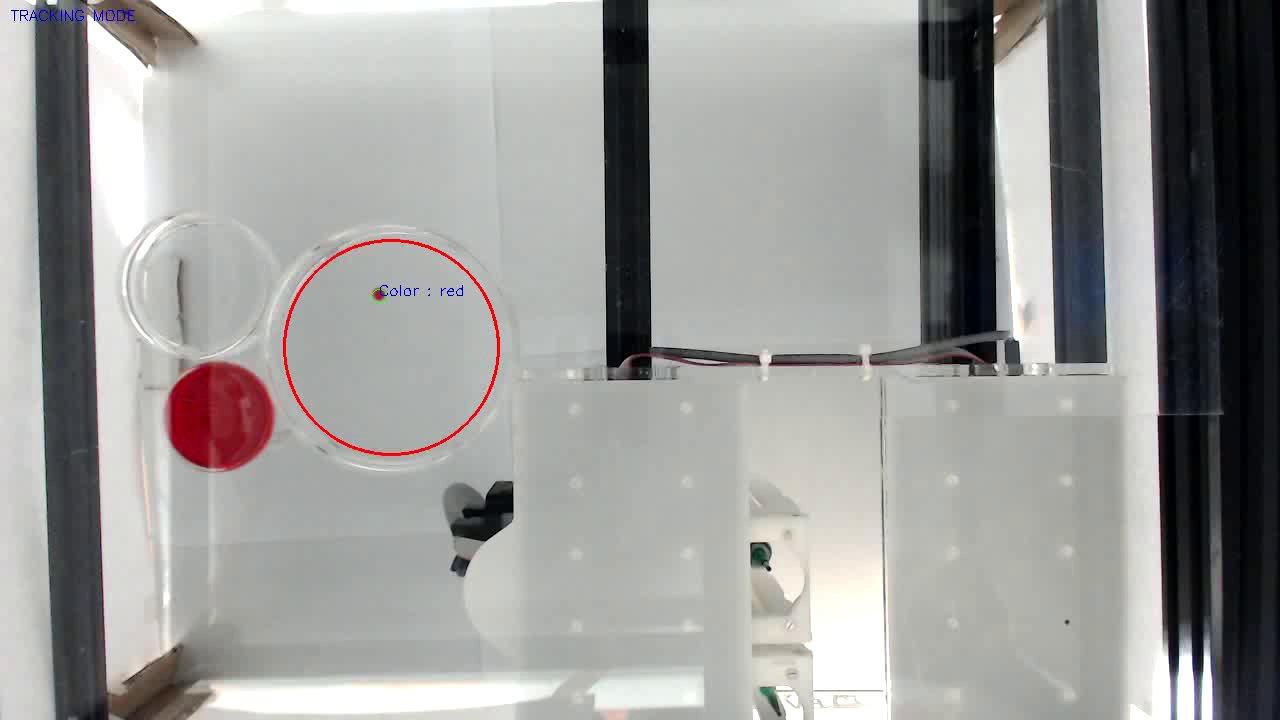
\includegraphics[width=8cm]{immagini/track.png}}
 	\hspace{2mm}   	
	{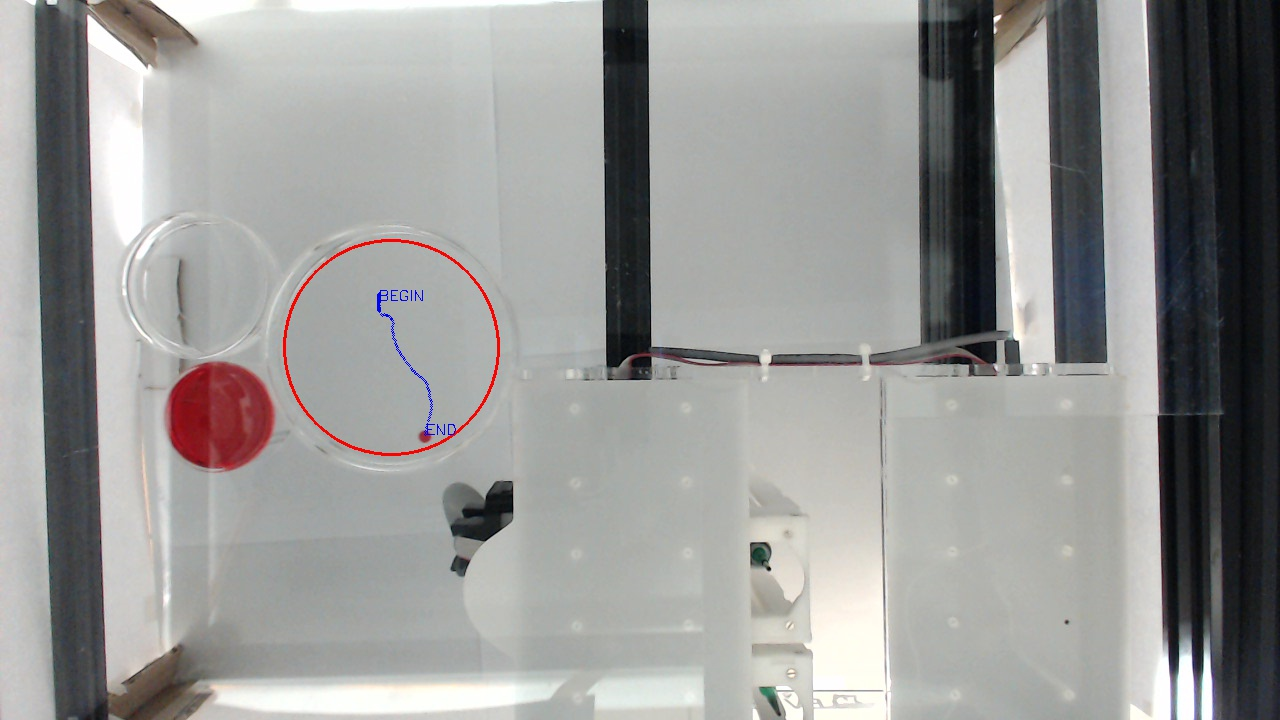
\includegraphics[width=8cm]{immagini/track_path.jpg}}
	\caption{tracking}
 	\end{figure}



\section{Dati}
Per trovare la combinazione migliore delle componenti nello spazio degli esperimenti si è applicata la funzione di adattamento per il movimento. Questa descrive la velocità media della droplet durante tutto l'esperimento ed è espressa in $1/s$. La funzione è stata applicata a due ripetizioni di ogni esperimento e la media è stata presa come valore di riferimento. La funzione è definita come:
\begin{equation*} 
\cfrac {\sqrt [ 2 ]{ { (A_{ x }-B_{ x }) }^{ 2 }+{ (A_{ y }-B_{ y }) }^{ 2 } } /\quad tempo }{ \sqrt [ 2 ]{ { (C_{ x }-B_{ x }) }^{ 2 }+{ (C_{ y }-B_{ y }) }^{ 2 }}} 
\end{equation*}
\\Dove: $A=(x,y)$ coordinate del primo punto in cui viene individuata la droplet, punto di inizio del percorso
$B=(x,y)$ coordinate del punto in cui viene inserito il sale NaCl
$C=(x,y)$ coordinate dell'ultimo punto in cui viene individuata la droplet, punto di fine percorso































      \chapter{Conclusioni e Sviluppi Futuri}
\vspace{0.5cm}
\label{cha:789}
Lorem ipsum dolor sit amet, consectetur adipiscing elit. Donec sed nunc orci. Aliquam nec nisl vitae sapien pulvinar dictum quis non urna. Suspendisse at dui a erat aliquam vestibulum. Quisque ultrices pellentesque pellentesque. Pellentesque egestas quam sed blandit tempus. Sed congue nec risus posuere euismod. Maecenas ut lacus id mauris sagittis egestas a eu dui. Class aptent taciti sociosqu ad litora torquent per conubia nostra, per inceptos himenaeos. Pellentesque at ultrices tellus. Ut eu purus eget sem iaculis ultricies sed non lorem. Curabitur gravida dui eget ex vestibulum venenatis. Phasellus gravida tellus velit, non eleifend justo lobortis eget. 


\section{Cras in aliquam quam, et}
\label{sec:456}
Lorem ipsum dolor sit amet, consectetur adipiscing elit. Donec sed nunc orci. Aliquam nec nisl vitae sapien pulvinar dictum quis non urna. Suspendisse at dui a erat aliquam vestibulum. Quisque ultrices pellentesque pellentesque. Pellentesque egestas quam sed blandit tempus. Sed congue nec risus posuere euismod. Maecenas ut lacus id mauris sagittis egestas a eu dui. Class aptent taciti sociosqu ad litora torquent per conubia nostra, per inceptos himenaeos. Pellentesque at ultrices tellus. Ut eu purus eget sem iaculis ultricies sed non lorem. Curabitur gravida dui eget ex vestibulum venenatis. Phasellus gravida tellus velit, non eleifend justo lobortis eget.


\subsection{Sed pulvinar placerat enim, a}
\label{sec:00456}
Lorem ipsum dolor sit amet, consectetur adipiscing elit. Donec sed nunc orci. Aliquam nec nisl vitae sapien pulvinar dictum quis non urna. Suspendisse at dui a erat aliquam vestibulum. Quisque ultrices pellentesque pellentesque. Pellentesque egestas quam sed blandit tempus. Sed congue nec risus posuere euismod. Maecenas ut lacus id mauris sagittis egestas a eu dui. Class aptent taciti sociosqu ad litora torquent per conubia nostra, per inceptos himenaeos. Pellentesque at ultrices tellus. Ut eu purus eget sem iaculis ultricies sed non lorem. Curabitur gravida dui eget ex vestibulum venenatis. Phasellus gravida tellus velit, non eleifend justo lobortis eget.


\section{Vivamus hendrerit imperdiet ex. Vivamus}
\label{sec:123}
Lorem ipsum dolor sit amet, consectetur adipiscing elit. Donec sed nunc orci. Aliquam nec nisl vitae sapien pulvinar dictum quis non urna. Suspendisse at dui a erat aliquam vestibulum. Quisque ultrices pellentesque pellentesque. Pellentesque egestas quam sed blandit tempus. Sed congue nec risus posuere euismod. Maecenas ut lacus id mauris sagittis egestas a eu dui. Class aptent taciti sociosqu ad litora torquent per conubia nostra, per inceptos himenaeos. Pellentesque at ultrices tellus. Ut eu purus eget sem iaculis ultricies sed non lorem. Curabitur gravida dui eget ex vestibulum venenatis. Phasellus gravida tellus velit, non eleifend justo lobortis eget.


	
      
  
      
      %fine del gruppo di "capitoli senza interruzione" di pagina
    % \endgroup


    % bibliografia in formato bibtex
    %
    % aggiunta del capitolo nell'indice
    \addcontentsline{toc}{chapter}{Bibliografia}
    % stile con ordinamento alfabetico in funzione degli autori
    \bibliographystyle{plain}
    \bibliography{biblio}
%%%%%%%%%%%%%%%%%%%%%%%%%%%%%%%%%%%%%%%%%%%%%%%%%%%%%%%%%%%%%%%%%%%%%%%%%%
%%%%%%%%%%%%%%%%%%%%%%%%%%%%%%%%%%%%%%%%%%%%%%%%%%%%%%%%%%%%%%%%%%%%%%%%%%
%% Nota
%%%%%%%%%%%%%%%%%%%%%%%%%%%%%%%%%%%%%%%%%%%%%%%%%%%%%%%%%%%%%%%%%%%%%%%%%%
%% Nella bibliografia devono essere riportati tutte le fonti consultate 
%% per lo svolgimento della tesi. La bibliografia deve essere redatta 
%% in ordine alfabetico sul cognome del primo autore. 
%% 
%% La forma della citazione bibliografica va inserita secondo la fonte utilizzata:
%% 
%% LIBRI
%% Cognome e iniziale del nome autore/autori, la data di edizione, titolo, casa editrice, eventuale numero dell’edizione. 
%% 
%% ARTICOLI DI RIVISTA
%% Cognome e iniziale del nome autore/autori, titolo articolo, titolo rivista, volume, numero, numero di pagine.
%% 
%% ARTICOLI DI CONFERENZA
%% Cognome e iniziale del nome autore/autori (anno), titolo articolo, titolo conferenza, luogo della conferenza (città e paese), date della conferenza, numero di pagine. 
%% 
%% SITOGRAFIA
%% La sitografia contiene un elenco di indirizzi Web consultati e disposti in ordine alfabetico. 
%% E’ necessario:
%%   Copiare la URL (l’indirizzo web) specifica della pagina consultata
%%   Se disponibile, indicare il cognome e nome dell’autore, il titolo ed eventuale sottotitolo del testo
%%   Se disponibile, inserire la data di ultima consultazione della risorsa (gg/mm/aaaa).    
%%%%%%%%%%%%%%%%%%%%%%%%%%%%%%%%%%%%%%%%%%%%%%%%%%%%%%%%%%%%%%%%%%%%%%%%%%
%%%%%%%%%%%%%%%%%%%%%%%%%%%%%%%%%%%%%%%%%%%%%%%%%%%%%%%%%%%%%%%%%%%%%%%%%%
    

    \titleformat{\chapter}
        {\normalfont\Huge\bfseries}{Allegato \thechapter}{1em}{}
    % sezione Allegati - opzionale
    \appendix
    \chapter{Titolo primo allegato}

Lorem ipsum dolor sit amet, consectetur adipiscing elit. Donec sed nunc orci. Aliquam nec nisl vitae sapien pulvinar dictum quis non urna. Suspendisse at dui a erat aliquam vestibulum. Quisque ultrices pellentesque pellentesque. Pellentesque egestas quam sed blandit tempus. Sed congue nec risus posuere euismod. Maecenas ut lacus id mauris sagittis egestas a eu dui. Class aptent taciti sociosqu ad litora torquent per conubia nostra, per inceptos himenaeos. Pellentesque at ultrices tellus. Ut eu purus eget sem iaculis ultricies sed non lorem. Curabitur gravida dui eget ex vestibulum venenatis. Phasellus gravida tellus velit, non eleifend justo lobortis eget. 

\section{Titolo}
Lorem ipsum dolor sit amet, consectetur adipiscing elit. Donec sed nunc orci. Aliquam nec nisl vitae sapien pulvinar dictum quis non urna. Suspendisse at dui a erat aliquam vestibulum. Quisque ultrices pellentesque pellentesque. Pellentesque egestas quam sed blandit tempus. Sed congue nec risus posuere euismod. Maecenas ut lacus id mauris sagittis egestas a eu dui. Class aptent taciti sociosqu ad litora torquent per conubia nostra, per inceptos himenaeos. Pellentesque at ultrices tellus. Ut eu purus eget sem iaculis ultricies sed non lorem. Curabitur gravida dui eget ex vestibulum venenatis. Phasellus gravida tellus velit, non eleifend justo lobortis eget. 

\subsection{Sottotitolo}
Lorem ipsum dolor sit amet, consectetur adipiscing elit. Donec sed nunc orci. Aliquam nec nisl vitae sapien pulvinar dictum quis non urna. Suspendisse at dui a erat aliquam vestibulum. Quisque ultrices pellentesque pellentesque. Pellentesque egestas quam sed blandit tempus. Sed congue nec risus posuere euismod. Maecenas ut lacus id mauris sagittis egestas a eu dui. Class aptent taciti sociosqu ad litora torquent per conubia nostra, per inceptos himenaeos. Pellentesque at ultrices tellus. Ut eu purus eget sem iaculis ultricies sed non lorem. Curabitur gravida dui eget ex vestibulum venenatis. Phasellus gravida tellus velit, non eleifend justo lobortis eget. 


\chapter{Titolo secondo allegato}

Lorem ipsum dolor sit amet, consectetur adipiscing elit. Donec sed nunc orci. Aliquam nec nisl vitae sapien pulvinar dictum quis non urna. Suspendisse at dui a erat aliquam vestibulum. Quisque ultrices pellentesque pellentesque. Pellentesque egestas quam sed blandit tempus. Sed congue nec risus posuere euismod. Maecenas ut lacus id mauris sagittis egestas a eu dui. Class aptent taciti sociosqu ad litora torquent per conubia nostra, per inceptos himenaeos. Pellentesque at ultrices tellus. Ut eu purus eget sem iaculis ultricies sed non lorem. Curabitur gravida dui eget ex vestibulum venenatis. Phasellus gravida tellus velit, non eleifend justo lobortis eget. 

\section{Titolo}
Lorem ipsum dolor sit amet, consectetur adipiscing elit. Donec sed nunc orci. Aliquam nec nisl vitae sapien pulvinar dictum quis non urna. Suspendisse at dui a erat aliquam vestibulum. Quisque ultrices pellentesque pellentesque. Pellentesque egestas quam sed blandit tempus. Sed congue nec risus posuere euismod. Maecenas ut lacus id mauris sagittis egestas a eu dui. Class aptent taciti sociosqu ad litora torquent per conubia nostra, per inceptos himenaeos. Pellentesque at ultrices tellus. Ut eu purus eget sem iaculis ultricies sed non lorem. Curabitur gravida dui eget ex vestibulum venenatis. Phasellus gravida tellus velit, non eleifend justo lobortis eget. 

\subsection{Sottotitolo}
Lorem ipsum dolor sit amet, consectetur adipiscing elit. Donec sed nunc orci. Aliquam nec nisl vitae sapien pulvinar dictum quis non urna. Suspendisse at dui a erat aliquam vestibulum. Quisque ultrices pellentesque pellentesque. Pellentesque egestas quam sed blandit tempus. Sed congue nec risus posuere euismod. Maecenas ut lacus id mauris sagittis egestas a eu dui. Class aptent taciti sociosqu ad litora torquent per conubia nostra, per inceptos himenaeos. Pellentesque at ultrices tellus. Ut eu purus eget sem iaculis ultricies sed non lorem. Curabitur gravida dui eget ex vestibulum venenatis. Phasellus gravida tellus velit, non eleifend justo lobortis eget. 




\end{document}
